%<*package>

\NewDocumentCommand \SimpleSystemTeX {d[]} {
    \IfValueTF {#1} {
        \str_case:nn {#1} {
            {rm} {
                \,$\mathrm{S^{imple}\sb{ystem}}$\textrm{\TeX}\,
            }
            {bf} {
                \,$\mathbf{S^{imple}\sb{ystem}}$\textbf{\TeX}\,
            }
        }
    } {
        \,$\mathrm{S^{imple}\sb{ystem}}$\textrm{\TeX}\,
    }
}

\ExplSyntaxOff

\def \plotsetting {
	\draw[
		black,
		ultra thick,
		domain = 0:360,
		smooth,
		samples = 100
	]
}
\NewDocumentCommand \SimpleSystem {} {
    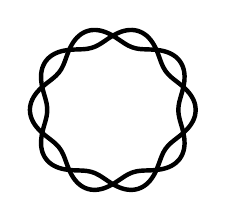
\begin{tikzpicture} [scale=0.3]
		\plotsetting
		plot (\x: {3.14159 - 0.36788 * cos (5 * \x)});
		\plotsetting
		plot (\x: {3.14159 + 0.36788 * cos (5 * \x)});
	\end{tikzpicture}
}
\NewDocumentCommand \SimpleSystemCover {m d[]} {
    \begin{center}%
	    \vspace*{\fill}%
	    \SimpleSystem%
        \par #1%
        \IfValueT {#2} {\par #2}%
	    \vspace*{\fill}%
    \end{center}%
}

\ExplSyntaxOn

%</package>